\documentclass[border=10pt]{standalone}

\usepackage{amsmath}
\usepackage{tikz}
\usepackage{pgfplots}
\begin{document}
%
% \tikzset{
% axis/.style={black, thick},
% wave/.style={green!25!black, opacity=.5, fill=green!70!black, thick}}
% %
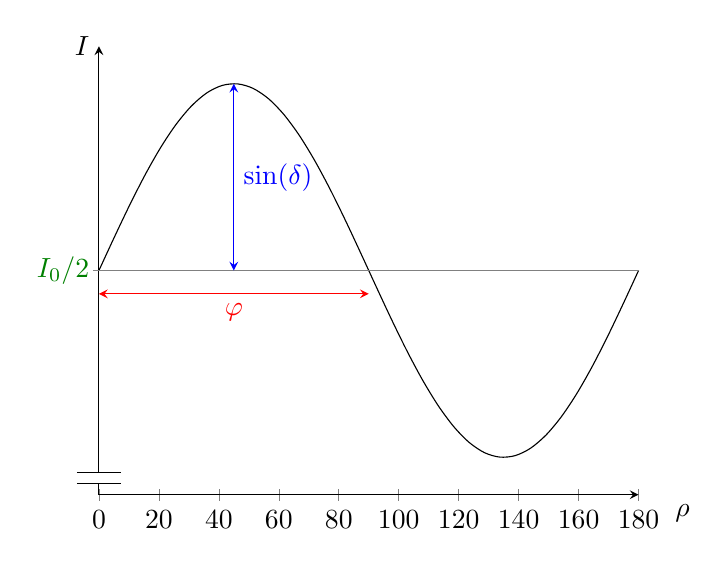
\begin{tikzpicture}[>=stealth]
\begin{axis}[
% hide axis,
clip=false,
axis lines=left,
enlargelimits=false,
xlabel=$\rho$,
ylabel=$I$,
% ylabel near ticks,s.right of origin
% xlabel near ticks,
every axis x label/.style={at={(rel axis cs:1.05,0)}, anchor=north west},
every axis y label/.style={at={(rel axis cs:0,1.0)}, anchor=east},
% every axis y label/.style={at={(current axis.north west)},above=2mm},
xtick={0,20,...,180},
xmin = 0, xmax = 180,
axis y discontinuity=parallel,
ymin = -1.2, ymax = 1.2,
ytick=\empty,
% ytick={-1,-0.5,...,1},
% yticklabels={$low$, $I_0/2$, $high$}
]
% \addplot[only marks,black,domain=0:170,samples=9,]{sin(2*x)};
\addplot[black,domain=0:180,samples=36,smooth]{sin(2*x)};
% 
\draw[help lines] (axis cs:-2,0) -- (axis cs:180,0);
\node[green!50!black, left] at (axis cs:0,0) {$I_0/2$};
\draw[red,<->] (axis cs:0,-0.125) -- (axis cs:90,-0.125) node[below,midway]{$\varphi$};
\draw[blue,<->] (axis cs:45,0) -- (axis cs:45,1) node[right,midway]{$\sin(\delta)$};
% \node[pin=0:{\texttt{xticklabel cs:0}}] at (xticklabel cs:1) {};
% 
\end{axis}
\end{tikzpicture}
% 
\end{document}